\documentclass[../../main]{subfiles}

\renewcommand\thesection{\arabic{section}}


\begin{document}

\section{Dedicated Coolers} \label{sec:}

The incubator area is sized at $50\si{cm} \times 50\si{cm} \times 80\si{cm}$. That
is almost $200\si{L}$ of air to cool. A single peltier module cannot do this properly.
So we are adding 4 more dedicated cooler to speed up the cooling process of the
incubator.

\subsection{Positioning of Dedicated Coolers}

% \begin{figure}
%     \centering
%     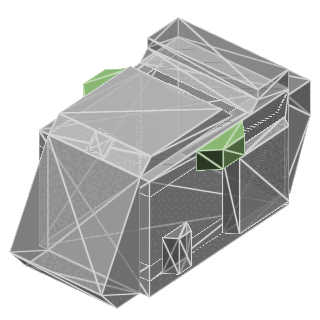
\includegraphics [
%         height = 0.2\textheight,
%         max width = \IGXMaxWidth,
%         max height = \IGXMaxHeight,
%         \IGXDefaultOptionalArgs,
%     ] {pics/ded_cooler_right.png}
%     \captionof{figure} {Positioning of dedicated coolers.}
%     \label{fig:}
% \end{figure}

\begin{center}
    \begin{minipage} {0.54\textwidth}
        Hot air rises and cold air sinks. So it is important to place
        the peltiers closer to the top of the incubator area. Figure
        \ref{fig:dedCoolerPlacement} shows the position of these four
        coolers. Inorder to dissipate the coldness from the cold side
        of the peltiers, each of them will have a DC fan forcing air
        towards the cold side. We are using the same 12V brushless DC fan
        that we have used in the core block. Refer figure \ref{fig:dc12VFan}.
        \vfill
    \end{minipage}
    \hfill
    \begin{minipage} {0.45\textwidth}
        \centering
        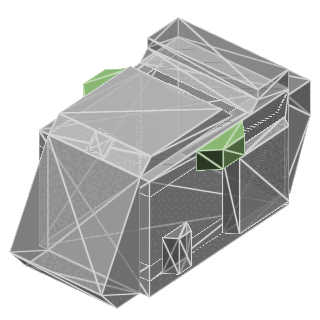
\includegraphics [
            height = 0.18\textheight,
            trim = {0 0 0 0},
            clip,
        ] {pics/ded_cooler_right.png}
        \captionof{figure} {Dedicated coolers.}
        \label{fig:dedCoolerPlacement}
    \end{minipage}
\end{center}

\end{document}
